% vim:fdm=marker:
\documentclass[]{beamer}                                                % {{{1
\setbeamertemplate{itemize item}{--}
\setbeamertemplate{navigation symbols}{}
\setbeamertemplate{footline}{
  \leavevmode
  \hbox{
    \begin{beamercolorbox}[wd=\paperwidth,ht=2.25ex,dp=1ex,right]{frame number}%
      \usebeamerfont{footline}
      \usebeamercolor[fg]{footline}
      \insertframenumber{}
      \hspace*{1ex}
    \end{beamercolorbox}
  }
}
\setbeamercovered{transparent=50}
\setbeamercolor{footline}{fg=black!60!white}
\setbeamercolor{alerted text}{fg=orange!80!black}
\setbeamerfont{alerted text}{family=\bfseries}
\usepackage[utf8]{inputenc}
\usepackage{amsmath,amsfonts,amssymb}
\usepackage{graphicx}
\graphicspath{{./}{img/}}

\usepackage[inline]{enumitem}
\setlist{
  topsep=0pt,itemsep=0pt, %
  labelsep=1ex, % between \item and text
  labelindent=0em,rightmargin=0em, % left most, right most border
  labelwidth=1em,leftmargin=!, % calculate left margin from label width
  font=\usebeamercolor[fg]{itemize item}\usebeamerfont{itemize item}\mdseries, % use beamer theme, but normal size
}
\setlist[itemize]{label=\usebeamertemplate{itemize item}}
\setlist[enumerate]{label=(\arabic*)}
\setlist[description]{style=nextline}

\usepackage{listings}
% \renewcommand{\ttdefault}{lmtt}
\lstset{
  escapechar=\%, % LaTeX between '%'
  % escapeinside=`', % LaTeX starting with ` ending with '
  % font/color
  backgroundcolor=,
  basicstyle=\ttfamily,
  basewidth=1.04ex,
  keywordstyle=\bfseries,
  identifierstyle=\bfseries,
  commentstyle=\sffamily\itshape,
  stringstyle=\sffamily,
  showstringspaces=false,
  % language definition
  language=,
  % interfaces
  emphstyle={[2]\slshape},
  emph={[2]
    % own
    Simulation,
    Controller,
    ResultListener,
    EstimatorListener,
    Differentiation,
    UpdateStep,
  },
}

\usepackage{tikz}
\usetikzlibrary{arrows}
\usetikzlibrary{calc}
\usetikzlibrary{shapes.multipart}
\usetikzlibrary{decorations.pathmorphing}
% layers
\pgfdeclarelayer{edgelayer}
\pgfdeclarelayer{nodelayer}
\pgfsetlayers{edgelayer,nodelayer,main}
% style
\tikzstyle{defline}=[line width=0.4pt]
\tikzstyle{defnode}=[defline,align=center,inner sep=1.4pt,font=\tiny]
\tikzstyle{defrectsplit}=[rectangle split,
rectangle split part align={center,left}, % align the box
every two node part/.style={align=left} % align the content inside a box
]
\tikzstyle{defedge}=[defline,draw=black,every node/.style={defnode,sloped,fill=white,fill opacity=1}]
\tikzstyle{defdeko}=[decorate,decoration={pre length=3pt,post length=6pt}]
\tikzstyle{defsnake}=[defdeko,decoration={snake,amplitude=2pt,segment length=4pt}]
% node styles
\tikzstyle{none}=[defnode]
\tikzstyle{note}=[defnode,font=\em\tiny\color{gray}]
% info
\tikzstyle{infoarrow}=[defedge,-latex]
\tikzstyle{infoborder}=[defedge,gray,line width=1.2pt,dashdotted]
\tikzstyle{infoprocess}=[defsnake,infoarrow]
\tikzstyle{infoprocesspos}=[infoprocess,dotted,gray,decoration={segment length=8pt}]
% uml styles
\tikzstyle{umlbox}=[defnode,rectangle,draw=black,fill=white]
\tikzstyle{umlnotebox}=[umlbox,defrectsplit,rectangle split parts=2]
\tikzstyle{umlhas}=[defedge,-open diamond,every node/.style={defnode,auto,pos=.1}]
\tikzstyle{umlisa}=[defedge,-open triangle 45]
% sequence style
\tikzstyle{seqinit}=[defnode,circle,fill=black,minimum width=4pt]
\tikzstyle{seqbox}=[umlbox]
\tikzstyle{seqobj}=[defedge,dashed]
\tikzstyle{seqcall}=[defedge,-latex]
\tikzstyle{seqreturn}=[defedge,dotted,-latex]
\tikzstyle{seqrunning1}=[draw=black,fill=gray,line width=.25pt,line cap=round,double distance=.8pt]
\tikzstyle{seqrunning2}=[seqrunning1,double distance=1.6pt]
\tikzstyle{seqloop}=[defedge,draw=gray,|-|]


\usepackage{tikz}
% animation needs [fragile] frames
% \foreach \pc in {1,2} {\only<+>{
%   \begin{scaletikzpicturetowidth}{.8\textwidth}
%     \input{name.tikz}
%   \end{scaletikzpicturetowidth}
% }}
\def\pc{1}
\tikzset{
  apply special/.style={special #1},
  % keyword: alert=SLIDE
  alert/.style={normal,apply special/.list/.expand once=alert_\pc,#1},
  normal/.style={
    0/.style={},
    1/.style={},
    2/.style={},
    3/.style={},
    4/.style={},
    5/.style={},
    6/.style={},
    7/.style={},
    8/.style={},
  },
  special alert_0/.style={0/.style={draw=orange!80!black,line width=0.6pt}},
  special alert_1/.style={1/.style={draw=orange!80!black,line width=0.6pt}},
  special alert_2/.style={2/.style={draw=orange!80!black,line width=0.6pt}},
  special alert_3/.style={3/.style={draw=orange!80!black,line width=0.6pt}},
  special alert_4/.style={4/.style={draw=orange!80!black,line width=0.6pt}},
  special alert_5/.style={5/.style={draw=orange!80!black,line width=0.6pt}},
  special alert_6/.style={6/.style={draw=orange!80!black,line width=0.6pt}},
  special alert_7/.style={7/.style={draw=orange!80!black,line width=0.6pt}},
  special alert_8/.style={8/.style={draw=orange!80!black,line width=0.6pt}},
  % keyword: uncover=SLIDE
  uncover/.style={covered,apply special/.list/.expand once=uncover_\pc,#1},
  covered/.style={
    1/.style={opacity=.6},
    2/.style={opacity=.6},
    3/.style={opacity=.6},
    4/.style={opacity=.6},
    5/.style={opacity=.6},
    6/.style={opacity=.6},
  },
  special uncover_1/.style={1/.style={opacity=1}},
  special uncover_2/.style={2/.style={opacity=1}},
  special uncover_3/.style={3/.style={opacity=1}},
  special uncover_4/.style={4/.style={opacity=1}},
  special uncover_5/.style={5/.style={opacity=1}},
  special uncover_6/.style={6/.style={opacity=1}},
}

% http://tex.stackexchange.com/questions/6388/how-to-scale-a-tikzpicture-to-textwidth
\usepackage{tikz}
\usepackage{environ}
\makeatletter
\newsavebox{\measure@tikzpicture}
\NewEnviron{scaletikzpicturetowidth}[1]{%
\def\tikz@width{#1}%
\def\tikzscale{1}\begin{lrbox}{\measure@tikzpicture}%
\BODY
\end{lrbox}%
\pgfmathparse{#1/\wd\measure@tikzpicture}%
\edef\tikzscale{\pgfmathresult}%
\BODY
}
\makeatother


\DeclareMathOperator*{\argmin}{argmin}
% }}}1

\title{RSienaCPP}
\author{Felix Schönenberger}
\institute{Department of Computer \& Information Science\\University of Konstanz}
\date{RSiena Developers Meeting\\Barcelona, 30 June 2014}

\def\scriptsize{\fontsize{7pt}{8pt}\selectfont}
\begin{document}
\begin{frame}                                                           % {{{1
  \titlepage
\end{frame}
\begin{frame}{Motivation}                                               % {{{1
  \begin{description}
    \item<1->[RSiena] Implementation of the stochastic actor-oriented model
      (SAOM)
    \item<2->[SAOM] Model supporting researchers understanding effects
      explaining network (co)evolution
  \end{description}
  \vfill
  \uncover<3->{(Perceived) Problems
    \begin{itemize}
      \item Slow (applicable for a few hundred actors)
        % ~1000 actors, 48 effects, 2 days
        % limitation on actors, assumptions of the model
        % strange behaviour on cluster
      \item High memory consumption
        % same set, 1GB per process
      \item Hard to maintain, extend
    \end{itemize}
  }
\end{frame}
\begin{frame}{Solutions}                                                % {{{1
  \begin{description}
    \item<1->[Theoretical] E.g. Settings model \vfill

    \item<2->[Practical]
      Migrate estimator from R to C++
      \begin{itemize}
        \item Reduce communication overhead
        \item Reduce memory overhead
        \item Clean modular redesign
      \end{itemize}
  \end{description}
\end{frame}
% \begin{frame}{Parts of RSiena}                                        % {{{1
%   \begin{center}
%     \begin{tikzpicture}[every node/.style={font=\scriptsize}]
%       \path[node distance=.3\textwidth]
%       node                 (theta0) {$\theta_t$}
%       node[right of=theta0] (sample) {$S(X_\text{sample})$}
%       node[right of=sample] (theta1) {$\theta_{t+1}$}
%       ;
%       \path[-latex]
%       (theta0.east) edge node[above]{sampling} (sample.west)
%       (sample.east) edge node[above]{update} (theta1.west)
%       ;
%       \draw[-latex]
%       (theta1.south)
%       -- ($(theta1)+(0,-.6)$)
%       -- ($(theta0)+(0,-.6)$)
%       -- (theta0.south)
%       ;
%       \node at ($(sample)+(0,-1)$) {$\theta : \text{model},
%       S(X_{\text{sample}}) : \text{statistics on sampled network}$};
%     \end{tikzpicture}
%   \end{center}
%   \begin{columns}[t]
%     \column<2->{.5\textwidth}
%     {\usebeamercolor[fg]{itemize item}
%     Sampling}
%     {\small
%       \begin{itemize}
%         \itemsep=-.2em
%         \item Draw networks from the model distribution
%         \item Code already in \texttt{C++}
%         \item Runtime depends on \#waves, \alert<6>{effects, \#actors}
%       \end{itemize}
%       \begin{itemize}
%         \itemsep=-.2em
%         \item<3-> Decreased sampling time $\to$ lower overall time
%       \end{itemize}
%     }
%     \column<4->{.5\textwidth}
%     {\usebeamercolor[fg]{itemize item}
%     \alert<8->{Estimation}}
%     {\small
%       \begin{itemize}
%         \itemsep=-.2em
%         \item Iteratively improve the model
%         \item Code in \texttt{R}
%         \item Runtime depends on \#waves, \alert<7>{\#effects, \#processes}
%       \end{itemize}
%       \begin{itemize}
%         \itemsep=-.2em
%         \item<5-> Reduce overhead
%         \item<5-> Towards standalone implementation
%         \item<5-> Modular
%       \end{itemize}
%     }
%   \end{columns}
%   % no real choice if the last decision is honored
%   % estimator not (asymptotically) faster
% \end{frame}
% \begin{frame}{RSienaCPP}                                                % {{{1
%   \begin{enumerate}
%     \item Migrate estimator from R to C++
%       \begin{itemize}
%         \item No algorithmic change
%         \item Statistically correct results
%       \end{itemize}
%     % \item \emph{Generalized Method of Moments}
%   \end{enumerate}
%   \vfill
%   % \pause
%   % {\usebeamercolor[fg]{itemize item}Outline}
%   % \begin{itemize}
%   %   \item Estimator
%   %   \item Parallelization
%   %   \item Result aggregation
%   % \end{itemize}
% \end{frame}
\begin{frame}{Estimator}                                                % {{{1
  Estimate parameters \quad $\widehat{\theta}$ s.t. $E_{\theta} [ S - s ] = 0$
  \vfill
  \uncover<2->{
    Robbins-Monro Estimator:
    \begin{description}[style=unboxed,labelindent=2em]
      \item[Phase 1] Approximate derivative
      \item[Phase 2] Update model
      \item[Phase 3] Test significance of effects
    \end{description}
  }
  \vfill
  \uncover<3->{
    A phase:
    \begin{enumerate}[labelindent=2em]
      \item Series of:
        \begin{itemize}
          \item (Parallel) simulations
          \item Aggregation of the results

            (e.g. sum up all derivatives)
        \end{itemize}
      \item Prepare next phase

        (e.g. prepare update step)
    \end{enumerate}
  }
  \vfill
  % \uncover<3->{
  %   "Replace" R by Eigen
  %   \begin{itemize}
  %     \item lightweight, pure template, linear algebra library
  %   \end{itemize}
  % }
\end{frame}
% \begin{frame}[fragile,t]{RSiena}                                      % {{{1
%   \def\fGlobal{2}
%   \def\fError{3}
%   \def\fExtend{4}
%   \def\fConcurrent{5}
%   \def\fCSide{6}
%   \begin{columns}[t]
%     \column{.5\textwidth}
%     \begin{semiverbatim}\scriptsize
% robmon <- function(\alert<\fGlobal>{z, x}, ...) \{
%   # initialize C++
%   \alert<\fConcurrent>{# setup cluster}
%   repeat \{
%     repeat \{
%       \alert<\fGlobal>{z <- phase1(z, ...);}
%       \alert<\fError>{if (!z\$OK || z\$Problem) \{
%         # error handling
%         break;
%       \}}
%       if (x\$nsub>0)
%         \alert<\fGlobal>{z <- phase2.1(z, ...);}
%       if (!z\$OK || Interrupt)
%         break;
%     \}
%     if (!z\$OK || Interrupt)
%       break;
%   \}
% \}
%     \end{semiverbatim}
%     \column{.5\textwidth}
%     \begin{semiverbatim}\scriptsize
% doIterations <- function(\alert<\fGlobal>{z, x}, ...) \{
%   repeat \{
%     \alert<\fExtend>{if (z\$int==1) \{}
%       zz <- \alert<\fCSide>{x\$FRAN(zsmall, xsmall)}
%       \alert<\fError>{if (!zz\$OK) \{
%         z\$OK <- zz\$OK
%         break
%       \}}
%     \alert<\fExtend>{\} else \{}
%       \alert<\fConcurrent>{zz <- clusterCall(z\$cl,
%         simstats0c, zsmall, xsmall)}
%       if (!all(zz\$OK)) \{
%         z\$OK <- FALSE
%         break
%       \}
%     \alert<\fExtend>{\}}
%     if (z\$nit >= z\$n2max)
%       break
%   \}
% \}
%     \end{semiverbatim}
%   \end{columns}
%   \only<\fGlobal->{
%     \begin{itemize}
%       \item%
%         \only<\fGlobal>{Global object holding all states}
%         \only<\fExtend>{One code instance, extension through new conditionals}
%         \only<\fError>{Error handling all over the place}
%         \only<\fConcurrent>{Concurrency built in the estimator}
%         \only<\fCSide>{Simulation objects on C++ side created every
%         iteration}
%     \end{itemize}
%   }
% \end{frame}
\begin{frame}[fragile,t]{Estimator}                                     % {{{1
  \def\fGlobal{3}
  \def\fPhase{4}
  \def\fEps{6}
  \def\fError{5}
  \vfill
  \begin{columns}
    \column<3->{.45\textwidth}
    \begin{semiverbatim}\scriptsize
# robmon.r
robmon <- function(\alert<\fGlobal>{z, x}, ...) \{
  x\$FRAN <- getFromNamespace(
               x\$FRANname, pkgname)
  repeat \{
    repeat \{
      \alert<\fGlobal>{z} <- \alert<\fPhase>{phase1}(\alert<\fGlobal>{z}, ...);
      if (\alert<\fError>{!z\$OK || z\$Problem}) \{
        break;
      \}
      \alert<\fEps>{if (z\$epsilonProblem) \{
        # error handling
        break;
      \}}
      if (x\$nsub>0)
        \alert<\fGlobal>{z} <- \alert<\fPhase>{phase2.1}(\alert<\fGlobal>{z}, ...);
      if (\alert<\fError>{!z\$OK || Interrupt})
        break;
    \}
    if (\alert<\fError>{!z\$OK || Interrupt})
      break;
  \}
\}
    \end{semiverbatim}%stopzone

    \column<2->{.55\textwidth}
    \foreach \pc in {0,1,2,3,4,5,6,7,8} {\only<+>{
        \begin{scaletikzpicturetowidth}{\textwidth}
          \begin{tikzpicture}[scale={\tikzscale}]
	\begin{pgfonlayer}{nodelayer}
		\node [style=umlnotebox,alert=3,alert=4] (0) at (0, 1) {
			\lstinline{Controller}\nodepart{two}
			\lstinline{run():bool}
		};
		\node [style=umlnotebox,alert=2] (1) at (0, 2) {
			\lstinline{Estimator}\nodepart{two}
			\lstinline{estimate()}
			\\\lstinline{approximateDerivative()}
			\\\lstinline{updateModel()}
			\\\lstinline{testModel()}
		};
		\node [style=umlnotebox,alert=6] (2) at (0, -1) {
			\lstinline{UpdateController}\nodepart{two}
			\lstinline{runSubphase(StopCondition)}
		};
		\node [style=umlnotebox,alert=5] (3) at (-0.5, -0) {
			\lstinline{DifferentiationController}\nodepart{two}
			\lstinline{rDerivative():MatrixXd}
		};
		\node [style=umlbox,alert=7] (4) at (0.5, -2) {\lstinline{StaticController}};
		\node [style=umlbox,alert=8] (5) at (2, 1.25) {\lstinline{Simulation}};
		\node [style=umlbox] (6) at (2, 0.75) {"Aggregator"};
	\end{pgfonlayer}
	\begin{pgfonlayer}{edgelayer}
		\draw [style=umlhas,alert=1] (0) to (1);
		\draw [style=umlisa] (2) to (0);
		\draw [style=umlisa,alert=1] (3) to (0);
		\draw [style=umlisa] (4) to (0);
		\draw [style=umlhas] (5) to (0);
		\draw [style=umlhas] (6) to node{*} (0);
	\end{pgfonlayer}
\end{tikzpicture}

        \end{scaletikzpicturetowidth}
    }}
  \end{columns}
  \vfill
\end{frame}
% \begin{frame}[t]{Phases 1}                                            % {{{1
%   \vfill
%   \begin{center}
%     \begin{scaletikzpicturetowidth}{\textwidth}
%       \input{phase1.tikz}
%     \end{scaletikzpicturetowidth}
%   \end{center}
%   \vfill
%   % \begin{itemize}
%   %   \item select differentiation method once

%   %   \item error handling might change differentiation again

%   %   \item Phase 3: same components, \lstinline{StaticController}

%   % \end{itemize}
%   \vfill
% \end{frame}
% \begin{frame}[t]{Phases 2}                                            % {{{1
%   \vfill
%   \begin{center}
%     \begin{scaletikzpicturetowidth}{.8\textwidth}
%       \input{phase2.tikz}
%     \end{scaletikzpicturetowidth}
%   \end{center}
%   \vfill
%   % \begin{itemize}
%   %   \item step chosen once in phase 1
%   % \end{itemize}
%   \vfill
% \end{frame}
% \begin{frame}[t]{Concurrent Processing}                               % {{{1
%   \vfill
%   \begin{center}
%     \begin{scaletikzpicturetowidth}{.8\textwidth}
%       \begin{tikzpicture}[scale={\tikzscale}]
	\begin{pgfonlayer}{nodelayer}
		\node [style=umlnotebox] (0) at (-1, 2.75) {
			\lstinline{Simulation}\nodepart{two}
			% \lstinline{addResultListener(Listener)}
			% \\\lstinline{addResultModificator(Modificator)}
			\lstinline{updateParameter(VectorXd)}
			\\\lstinline{nSimulations():int}
			\\\lstinline{simulate()}
		};
		\node [style=umlbox,alert=1,alert=2] (1) at (0, 1) {\lstinline{ForwardSimulation}};
		\node [style=umlbox,alert=2,alert=3] (2) at (0.5, -0) {\lstinline{MPIForwardSimulation}};
		\node [style=umlbox,alert=1] (3) at (-2, 0.5) {\lstinline{MaxLikeSimulation}};
		\node [style=umlbox] (4) at (0, -1) {\lstinline{EpochSimulation}};
		\node [style=umlbox] (5) at (-2, -1) {\lstinline{MLSimulation}};
	\end{pgfonlayer}
	\begin{pgfonlayer}{edgelayer}
		\draw [style=umlisa] (1) to (0);
		\draw [style=umlisa] (3) to (0);
		\draw [style=umlisa] (2) to (1);
		\draw [style=umlhas] (4) to (1);
		\draw [style=umlhas] (5) to (3);
	\end{pgfonlayer}
\end{tikzpicture}

%     \end{scaletikzpicturetowidth}
%   \end{center}
%   \vfill
%   \begin{itemize}
%     \item simple interface, takes and returns C++ vectors

%     \item estimator is independent of the parallelization

%   \end{itemize}
% \end{frame}
\begin{frame}[fragile,t]{Parallelization}                               % {{{1
  \vfill
  \begin{center}
    \foreach \pc in {1,2} {\only<+>{
        \begin{scaletikzpicturetowidth}{.8\textwidth}
          \begin{tikzpicture}[scale={\tikzscale}]
	\begin{pgfonlayer}{nodelayer}
		\node [style=none] (0) at (-5, 0.5) {R};
		\node [style=none] (1) at (-5, -0.75) {C};
		\node [style=none] (2) at (-2, 0.5) {R};
		\node [style=none] (3) at (-3, -0.75) {C};
		\node [style=none] (4) at (-3, -0) {R};
		\node [style=none,uncover=2] (5) at (1, -0.75) {C};
		\node [style=none,uncover=2] (6) at (1.5, 0.5) {R};
		\node [style=none,uncover=2] (7) at (2, -0.75) {C};
		\node [style=none] (8) at (-6.5, -0) {R process};
		\node [style=none] (9) at (-6.5, -0.75) {C thread};
		\node [style=none] (10) at (-5, 1.5) {Single core};
		\node [style=none] (11) at (-2, 1.5) {Forking};
		\node [style=none,uncover=2] (12) at (1.5, 1.5) {Threading};
		\node [style=none] (13) at (-1, -0) {R};
		\node [style=none] (14) at (-1, -0.75) {C};
	\end{pgfonlayer}
	\begin{pgfonlayer}{edgelayer}
		\draw [style=infoarrow] (0) to (1);
		\draw [style=infoarrow,uncover=2] (6) to (5);
		\draw [style=infoarrow,uncover=2] (6) to (7);
		\draw [style=infoarrow] (4) to (3);
		\draw [style=infoarrow] (2) to (4);
		\draw [style=infoarrow] (13) to (14);
		\draw [style=infoarrow] (2) to (13);
	\end{pgfonlayer}
\end{tikzpicture}

        \end{scaletikzpicturetowidth}
    }}
  \end{center}
  \vfill
  \begin{itemize}
    \item Forking: one C thread per R process
      \begin{itemize}
        \item RSiena: \texttt{parallel} R-package
        \item RSienaCPP: Message Passing Interface (MPI)
      \end{itemize}
    \item<2> Threading/hybrid: multiple C threads per R process
      \begin{itemize}
        \item RSienaCPP: OpenMP
      \end{itemize}
  \end{itemize}
  \vfill
\end{frame}
\begin{frame}[fragile,t]{Parallelization}                               % {{{1
  \def\fSingle{1}
  \def\fIfGlobal{2}
  \def\fCluster{3}
  \vspace{1.5em}
  \begin{columns}
    \column{.5\textwidth}
    \begin{semiverbatim}\scriptsize
# phase3.r
doPhase1or3Iterations <- function(z, x, ...)
\{
  for (nit in nits) \{
    \alert<\fIfGlobal>{if (\alert<\fIfGlobal>{z\$int}==1) \{}
      \alert<\fSingle>{zz <- x\$FRAN(zsmall, xsmall)}
      if (!zz\$OK) \{
        # ...
      \}
    \alert<\fIfGlobal>{\} else \{}
      \alert<\fCluster>{zz <- clusterCall(z\$cl,
        simstats0c, zsmall, xsmall)}
      if (!all(zz\$OK)) \{
        # ...
      \}
    \alert<\fIfGlobal>{\}}
    # process results
  \}
\}
    \end{semiverbatim}%stopzone

    \column{.5\textwidth}
    \foreach \pc in {1,2,3} {\only<+>{
        \begin{scaletikzpicturetowidth}{.8\textwidth}
          \begin{tikzpicture}[scale={\tikzscale}]
	\begin{pgfonlayer}{nodelayer}
		\node [style=umlnotebox] (0) at (-1, 2.75) {
			\lstinline{Simulation}\nodepart{two}
			% \lstinline{addResultListener(Listener)}
			% \\\lstinline{addResultModificator(Modificator)}
			\lstinline{updateParameter(VectorXd)}
			\\\lstinline{nSimulations():int}
			\\\lstinline{simulate()}
		};
		\node [style=umlbox,alert=1,alert=2] (1) at (0, 1) {\lstinline{ForwardSimulation}};
		\node [style=umlbox,alert=2,alert=3] (2) at (0.5, -0) {\lstinline{MPIForwardSimulation}};
		\node [style=umlbox,alert=1] (3) at (-2, 0.5) {\lstinline{MaxLikeSimulation}};
		\node [style=umlbox] (4) at (0, -1) {\lstinline{EpochSimulation}};
		\node [style=umlbox] (5) at (-2, -1) {\lstinline{MLSimulation}};
	\end{pgfonlayer}
	\begin{pgfonlayer}{edgelayer}
		\draw [style=umlisa] (1) to (0);
		\draw [style=umlisa] (3) to (0);
		\draw [style=umlisa] (2) to (1);
		\draw [style=umlhas] (4) to (1);
		\draw [style=umlhas] (5) to (3);
	\end{pgfonlayer}
\end{tikzpicture}

        \end{scaletikzpicturetowidth}
    }}
  \end{columns}
\end{frame}
\begin{frame}[fragile,t]{Parallelization}                               % {{{1
  \def\fIf{1}
  \def\fSim{2}
  \vspace{1.5em}
  \begin{columns}
    \column{.5\textwidth}
    \begin{semiverbatim}\scriptsize
# phase3.r
doPhase1or3Iterations <- function(z, x, ...)
\{
  for (nit in nits) \{
    if (z\$int==1) \{
      zz <- x\$FRAN(zsmall, xsmall)
      if (!zz\$OK) \{
        # ...
      \}
    \} else \{
      zz <- clusterCall(z\$cl,
        simstats0c, zsmall, xsmall)
      if (!all(zz\$OK)) \{
        # ...
      \}
    \}
    \alert<\fSim>{# process results}
  \}
\}
    \end{semiverbatim}%stopzone

    \column{.5\textwidth}
    \begin{semiverbatim}\scriptsize
// RInterface.cpp
Simulation* pSim = 0;
\alert<\fIf>{if} (maxLike) \{
  pSim = new MetropolisHastingsSimulation(
             pModel, pData);
\} \alert<\fIf>{else if} (/* mpi cluster */) \{
  pSim = new MPIStatisticsSimulation(
             pModel, pData, nThreads);
\} \alert<\fIf>{else} \{
  pSim = new StatisticsSimulation(
             pModel, pData, nThreads);
\}
Estimator con(\alert<\fIf>{*pSim}, ...);
con.estimate();
    \end{semiverbatim}
  \end{columns}

  % \begin{columns}[t]
  %   \column{.55\textwidth}
  %   \begin{itemize}
  %     \item Version for phase 1\&3, phase 2
  %     \item Decide in each iteration
  %   \end{itemize}

  %   \column{.55\textwidth}
  %   \begin{itemize}
  %     \item Decide once
  %     \item Estimator is independent
  %   \end{itemize}
  % \end{columns}
\end{frame}
\begin{frame}[fragile,t]{Result aggregation}                            % {{{1
  \vfill
  \begin{columns}
    \column<1>{.4\textwidth}
    \begin{itemize}
      \item Series of simulations:

        $ s(X_i) $ $i$-th statistics

      \item Aggregation:

        $sf = \left(\begin{array}{c}s(X_1)'\\\vdots\\s(X_n)'\end{array}\right)$

    \end{itemize}

    \column<2>{.5\textwidth}
    \begin{scaletikzpicturetowidth}{\textwidth}
      \begin{tikzpicture}[scale={\tikzscale}]
	\begin{pgfonlayer}{nodelayer}
		\node [style=umlnotebox] (0) at (0, 1) {
			\lstinline{Controller}\nodepart{two}
			\lstinline{run():bool}
		};
		\node [style=umlnotebox, alert=6] (1) at (-1.25, -0) {
			\lstinline{Simulation}\nodepart{two}
			\lstinline{addResultListener(.)}
		};
		\node [style=umlnotebox] (2) at (1.25, -0) {
			"Aggregator"\nodepart{two}
			\lstinline{onResult(Result)}
		};
		\node [style=umlbox] (3) at (0, -0.5) {\lstinline{Result}};
		\node [style=none] (4) at (0, -0) {};
	\end{pgfonlayer}
	\begin{pgfonlayer}{edgelayer}
		\draw [style=umlhas] (1) to (0);
		\draw [style=umlhas] (2) to node[pos=.4]{*} (0);
		\draw [style=seqreturn] (1) to (2);
		\draw [dotted] (4.center) to (3);
	\end{pgfonlayer}
\end{tikzpicture}

    \end{scaletikzpicturetowidth}
  \end{columns}
  \vfill
  \uncover<3>{
    \begin{description}[style=unboxed]
      \item[Listener design pattern:] Event driven one-to-many communication
      \item[Publisher:] Distributes event to registered listeners
      \item[Listener:] Interface defining \lstinline{onEvent(Event)} method
    \end{description}
  }
  \vfill
\end{frame}
\begin{frame}[fragile,t]{Result aggregation}                            % {{{1
  \def\fSimulation{2}
  \def\fIfPara{3}
  \def\fIfDeriv{4}
  \vfill
  \begin{columns}
    \column<2->{.5\textwidth}
    \begin{semiverbatim}\scriptsize
# phase3.r
\alert<\fSimulation>{# zz <- simulation(z)}
\alert<\fIfPara>{if (z\$int==1) \{}
  fra <- colSums(zz\$fra)
  z\$sf[z\$nit, ] <- fra
\alert<\fIfPara>{\} else \{}
\alert<\fIfPara>{\}}
\alert<\fIfDeriv>{if (x\$maxlike) \{} # ...
\alert<\fIfDeriv>{\} else if (z\$FinDiff.method) \{} # ...
\alert<\fIfDeriv>{\} else \{}
  \alert<\fIfPara>{if (int==1) \{} # ...
  \alert<\fIfPara>{\} else \{} # ...
  \alert<\fIfPara>{\}}
\alert<\fIfDeriv>{\}}
    \end{semiverbatim}%stopzone

    \column{.5\textwidth}
    \foreach \pc in {0,1,2,3} {\only<+>{
        \begin{scaletikzpicturetowidth}{\textwidth}
          \begin{tikzpicture}[scale={\tikzscale}]
	\begin{pgfonlayer}{nodelayer}
		\node [style=umlnotebox,alert=1] (0) at (0, -1) {
			\lstinline{Simulation}\nodepart{two}
			\lstinline{addResultListener(listener)}
			\\\lstinline{simulate()}
		};
		\node [style=umlnotebox] (1) at (0, 1.5) {
			\lstinline{Controller}\nodepart{two}
			\lstinline{addEstimatorListener(listener)}
			\\\lstinline{run()}
		};
		\node [style=umlnotebox] (2) at (2.5, 0.25) {
			\lstinline{EstimatorListener}\nodepart{two}
			\lstinline{initializePhase()}
			\\\lstinline{finalizePhase(int)}
		};
		\node [style=umlnotebox] (3) at (2.5, -2.25) {
			\lstinline{ResultListener}\nodepart{two}
			\lstinline{needs():vector<ResultType>}
			\\\lstinline{onResult(Result)}
		};
		\node [style=umlnotebox,alert=2] (4) at (0, -3.5) {
			\lstinline{Result}\nodepart{two}
			\lstinline{pStatistics():vector<VectorXd>*}
			\\\lstinline{// ...}
		};
		\node [style=umlbox,alert=3] (5) at (3, -1) {"Aggregator"};
	\end{pgfonlayer}
	\begin{pgfonlayer}{edgelayer}
		\draw [style=umlhas] (0) to (1);
		\draw [style=umlhas] (2) to node[pos=.4]{*} (1);
		\draw [style=umlhas] (3) to node[pos=.4]{*} (0);
		\draw [style=umlhas] (4) to (0);
		\draw [style=umlisa] (5) to (2);
		\draw [style=umlisa] (5) to (3);
	\end{pgfonlayer}
\end{tikzpicture}

        \end{scaletikzpicturetowidth}
    }}
  \end{columns}
  \vfill
\end{frame}
\begin{frame}[fragile,t]{Result aggregation}                            % {{{1
  \def\fInit{1}
  \def\fReg{2}
  \def\fRun{3}
  \def\fUnreg{4}
  \def\fAccess{5}
  \vfill
  \begin{columns}
    \column{.5\textwidth}
    \begin{semiverbatim}\scriptsize
# phase3.r
# zz <- simulation(z)
if (z\$int==1) \{
  fra <- colSums(zz\$fra)
  z\$sf[z\$nit, ] <- fra
\} else \{
\}
if (x\$maxlike) \{ # ...
\} else if (z\$FinDiff.method) \{ # ...
\} else \{
  if (int==1) \{ # ...
  \} else \{ # ...
  \}
\}
    \end{semiverbatim}%stopzone

    \column{.5\textwidth}
    \begin{semiverbatim}\scriptsize
// Estimator.cpp
StaticController c(simulation, iterations);
StatisticCollector stats(/* ... */);
Differentiation* diff = \alert<\fInit>{/* ... */};

// register components
\alert<\fReg>{c.addListener(&stats);}
\alert<\fReg>{c.addListener(diff);}

\alert<\fRun>{c.run();} // run complete phase

\alert<\fUnreg>{c.removeListener(diff);}
\alert<\fUnreg>{c.removeListener(&stats);}

// access aggregated results
MatrixXd dfra = \alert<\fAccess>{diff->rDerivative()};
MatrixXd sf = \alert<\fAccess>{stats.rStatistics()};
    \end{semiverbatim}
  \end{columns}
  \vfill

  % \begin{columns}[t]
  %   \column{.55\textwidth}
  %   \begin{itemize}
  %     \item Version for phase 1\&3, phase 2
  %     \item Runs in each iteration
  %   \end{itemize}

  %   \column{.55\textwidth}
  %   \begin{itemize}
  %     \item Independent components
  %     \item Choose components once
  %   \end{itemize}

  % \end{columns}
\end{frame}
\begin{frame}[fragile,t]{Result aggregation}                            % {{{1
  \def\fNeed{1}
  \def\fInitialize{2}
  \def\fResult{3}
  \vfill
  \begin{columns}
    \column{.45\textwidth}
    \begin{semiverbatim}\scriptsize
# phase3.r
# zz <- simulation(z)
if (z\$int==1) \{
  fra <- colSums(zz\$fra)
  z\$sf[z\$nit, ] <- fra
\} else \{
\}
if (x\$maxlike) \{ # ...
\} else if (z\$FinDiff.method) \{ # ...
\} else \{
  if (int==1) \{ # ...
  \} else \{ # ...
  \}
\}
    \end{semiverbatim}%stopzone

    \column{.55\textwidth}
    \begin{semiverbatim}\scriptsize
// StatisticCollector.cpp
vector<ResultType>& StatisticCollector::\alert<\fNeed>{needs}() \{
static vector<ResultType> needs(1, \alert<\fNeed>{STATISTICS});
  return needs;
\}
void StatisticCollector::\alert<\fInitialize>{initializePhase}() \{
  \alert<\fInitialize>{lStatistics.clear();}
\}
void StatisticCollector::\alert<\fResult>{onResults}(
    const Result& rResults) \{
  for (itr it = rResults.pStatistics()->begin();
      it != rResults.pStatistics()->end(); ++it) \{
    \alert<\fResult>{addStatistics(*it);}
  \}
\}
    \end{semiverbatim}
  \end{columns}
  \vfill

  % \begin{columns}[t]
  %   \column{.55\textwidth}
  %   \begin{itemize}
  %     \item Access global objects
  %     \item Check what should be there
  %   \end{itemize}

  %   \column{.55\textwidth}
  %   \begin{itemize}
  %     \item Auto build result type set
  %   \end{itemize}

  % \end{columns}
\end{frame}
% \begin{frame}[fragile,t]{RSiena 'dolby' extension}                    % {{{1
%   \def\fGlobal{2}
%   \def\fConditional{3}
%   \def\fOrNot{4}
%   \begin{columns}[t]
%     \column{.5\textwidth}
%     \begin{semiverbatim}\scriptsize
% robmon <- function(...) \{
%   \alert<\fConditional>{if (\alert<\fGlobal>{x\$dolby}) \{}
%     z\$n1 <- max(z\$n1, 50)
%   \alert<\fConditional>{\}}
% \}
% phase1.2<- function(...) \{
%   \alert<\fOrNot>{# for dolby option
%   z\$regrCoef <- rep(0, z\$pp)}
% \}
%     \end{semiverbatim}
%     \column{.5\textwidth}
%     \begin{semiverbatim}\scriptsize
% doIterations <- function(...) \{
%   \alert<\fConditional>{if (x\$dolby) \{}
%     # ...
%   \alert<\fConditional>{\}}
%   if (z\$int==1) \{
%     zz <- x\$FRAN(zsmall, xsmall)
%     # test !zz\$OK
%     \alert<\fConditional>{if (x\$dolby) \{}
%       # ...
%     \alert<\fConditional>{\}}
%   \} else \{
%     # clusterCall
%     \alert<\fConditional>{if (x\$dolby) \{}
%       # ...
%     \alert<\fConditional>{\} else \{}
%       # ...
%     \alert<\fConditional>{\}}
%     # test !all(zz\$OK)
%   \}
% \}
%     \end{semiverbatim}
%   \end{columns}
%   \only<\fGlobal->{
%     \begin{itemize}
%       \item%
%         \only<\fGlobal>{Modify the global objects}
%         \only<\fConditional>{Add conditionals}
%         \only<\fOrNot>{Or don't and waste space}
%     \end{itemize}
%   }
% \end{frame}
% \begin{frame}[t]{RSienaCPP 'dolby' extension}                         % {{{1
%   \vfill
%   \begin{center}
%     \begin{scaletikzpicturetowidth}{.7\textwidth}
%       \begin{tikzpicture}[scale={\tikzscale}]
	\begin{pgfonlayer}{nodelayer}
		\node [style=umlbox] (0) at (-2, 1.25) {\lstinline{DifferentiationController}};
		\node [style=umlnotebox] (1) at (-2, 0.25) {
			\lstinline{ScoreCollector}\nodepart{two}
			\lstinline{// needs [SCORES]}
			\\\lstinline{rScores():MatrixXd}
		};
		\node [style=umlbox] (2) at (2, 1.25) {\lstinline{UpdateController}};
		\node [style=umlnotebox] (3) at (2, 0.25) {
			\lstinline{DolbyModificator}\nodepart{two}
			\lstinline{// needs [SCORES,S-s]}
			\\\lstinline{rRegressionCoefficient():VectorXd}
			\\\lstinline{onResult(Result)}
		};
		\node [style=umlbox] (4) at (0, 2) {\lstinline{GMMEstimator}};
	\end{pgfonlayer}
	\begin{pgfonlayer}{edgelayer}
		\draw [style=umlhas] (1) to (0);
		\draw [style=umlhas] (3) to (2);
		\draw [style=umlhas] (2) to (4);
		\draw [style=umlhas] (0) to (4);
	\end{pgfonlayer}
\end{tikzpicture}
%     \end{scaletikzpicturetowidth}
%   \end{center}
%   \vfill
%   \begin{itemize}
%     \item \lstinline{ScoreCollector}: Collect scores values of phase 1
%     \item \lstinline{DolbyModificator}: Listener with write access to \lstinline{Result}
%   \end{itemize}
%   \vfill
% \end{frame}
% \begin{frame}[t]{Redesign}                                            % {{{1
%   \begin{center}
%     \begin{tikzpicture}
%       \node[anchor=south west,inner sep=0] at (0,0)
%       {\includegraphics[width=.8\textwidth]{class}};
%       % controller
%       \path<-1>[fill=white,opacity=.6] (0,5.25) rectangle (6,6);
%       \path<2->[fill=white,opacity=.0] (0,5.25) rectangle (6,6);
%       % simulation
%       \path<-2>[fill=white,opacity=.6] (0,0) rectangle (2,3);
%       \path<3->[fill=white,opacity=.0] (0,0) rectangle (2,3);
%       % rob mon
%       \path<-3>[fill=white,opacity=.6] (0,3) rectangle (6,5.25);
%       \path<4->[fill=white,opacity=.0] (0,3) rectangle (6,5.25);
%       % mom, diff
%       \path<-4>[fill=white,opacity=.6] (2,0) rectangle (9,3);
%       \path<5->[fill=white,opacity=.0] (2,0) rectangle (9,3);
%     \end{tikzpicture}
%   \end{center}
%   \only<2-4>{
%     \begin{itemize}
%       \item%
%         \only<2>{Controller: Setup components, error handling}
%         \only<3>{Simulation: Hides concurrency}
%         \only<4>{Estimator: Unaware of both}
%     \end{itemize}
%   }
% \end{frame}
% \begin{frame}[fragile,t]{RSiena 'dolby' extension}                    % {{{1
%   \def\fGlobal{2}
%   \def\fConditional{3}
%   \def\fOrNot{4}
%   \begin{columns}[t]
%     \column{.5\textwidth}
%     \begin{semiverbatim}\scriptsize
% robmon <- function(...) \{
%   \alert<\fConditional>{if (\alert<\fGlobal>{x\$dolby}) \{}
%     z\$n1 <- max(z\$n1, 50)
%   \alert<\fConditional>{\}}
% \}
% phase1.2<- function(...) \{
%   \alert<\fOrNot>{# for dolby option
%   z\$regrCoef <- rep(0, z\$pp)}
% \}
%     \end{semiverbatim}
%     \column{.5\textwidth}
%     \begin{semiverbatim}\scriptsize
% doIterations <- function(...) \{
%   \alert<\fConditional>{if (x\$dolby) \{}
%     # ...
%   \alert<\fConditional>{\}}
%   if (z\$int==1) \{
%     zz <- x\$FRAN(zsmall, xsmall)
%     # test !zz\$OK
%     \alert<\fConditional>{if (x\$dolby) \{}
%       # ...
%     \alert<\fConditional>{\}}
%   \} else \{
%     # clusterCall
%     \alert<\fConditional>{if (x\$dolby) \{}
%       # ...
%     \alert<\fConditional>{\} else \{}
%       # ...
%     \alert<\fConditional>{\}}
%     # test !all(zz\$OK)
%   \}
% \}
%     \end{semiverbatim}
%   \end{columns}
%   \only<\fGlobal->{
%     \begin{itemize}
%       \item%
%         \only<\fGlobal>{Modify the global objects}
%         \only<\fConditional>{Add conditionals}
%         \only<\fOrNot>{Or don't and waste space}
%     \end{itemize}
%   }
% \end{frame}
% \begin{frame}[fragile,t]{Redesign 'dolby' extension}                  % {{{1
%   \begin{center}
%     \begin{tikzpicture}
%       \node[anchor=south west,inner sep=0] at (0,0)
%       {\includegraphics[width=.16\textwidth]{class-dolby}};
%       \path<-1>[fill=white,opacity=.6] (0,0) rectangle (1.2,1.5);
%       \path<2->[fill=white,opacity=.0] (0,0) rectangle (1.2,1.5);
%     \end{tikzpicture}
%   \end{center}
%   \begin{semiverbatim}\scriptsize\uncover<3->{
% void MoMDolby::phase1(const int n1) \{
%   MoM::phase1(n1);

%   lRegrCoef = VectorXd(rSimulation().nEffects());
%   for (int i = 0; i < rSimulation().nEffects(); ++i) \{
%     lRegrCoef[i] = covariance(lStatsFull.col(i), lScoresFull.col(i))
%                      / variance(lScoresFull.col(i));
%   \}
% \}
%   }\end{semiverbatim}
% \end{frame}
% \begin{frame}{Further extensions}                                     % {{{1
%   Settings model
%    - RSiena
%      - Settings are a list of strings naming the covariate settings,
%        primary and universal setting are identified by number.
%      - Calculations added to the one code that does all.
%    - Draft
%      - Setting is an object providing the actors available.
%   GMOM (calculating additional statistics, grouped by weighting)
%    - RSiena
%      - %(what would they do)
%    - Draft
%      - %(what would we do)
% \end{frame}
% \begin{frame}[fragile]{Redesign}                                      % {{{1
%   \vfill
%   \vfill
%   \begin{itemize}
%     \item<4-> Pros
%       \begin{itemize}
%         \item Modular
%         \item Encapsulated concurrent processing
%         \item Threading
%       \end{itemize}

%     \item<5-> Cons
%       \begin{itemize}
%         \item Same memory consumption (per process)
%         \item No GUI
%       \end{itemize}

%   \end{itemize}
%   \vfill
% \end{frame}
\begin{frame}[fragile]{RSienaCPP}                                       % {{{1
  \begin{columns}[t]
    \column{.5\textwidth}
    Generalized Method of Moments
    \begin{itemize}
      \item Model, R, new effect type
      \item Estimator
        \begin{itemize}
          \item Non-square derivative
          \item Update step
        \end{itemize}
    \end{itemize}
    Logging
    \begin{itemize}
      \item Levels, filter, appender
      \item C++/R
    \end{itemize}
    Documentation
    \begin{itemize}
      \item Referencing R names/locations
      \item Rd, classdesign
    \end{itemize}
    Libraries
    \begin{itemize}
      \item Eigen (lina)
      \item MPI (cluster), OpenMP (threads)
      \item Automatic build configuration
    \end{itemize}

    \column{.5\textwidth}
    Evaluation
    \begin{itemize}
      \item Statistically correct results
      \item (Reduced overhead)
    \end{itemize}
    Litte change for users
    \begin{semiverbatim}\scriptsize
  require(RSienaCPP) # require(RSiena)
  siena07(model, data, ...)
  sienacpp(model, data, ...)
  # +/- some cluster/logging parameters
    \end{semiverbatim}\vspace{-.6em}
    \vspace{5em}
    Things not yet implemented
    \begin{itemize}
      \item Gui (progress bar)
      \item ML parallelization scheme
      \item Threaded RNG
      \item R side utilities (GMM)
    \end{itemize}

  \end{columns}
\end{frame}
% \begin{frame}[fragile]{Conclusion}                                      % {{{1
%   \vfill
%   Resumé:
%   \begin{itemize}
%     \item Modular redesing
%       \begin{itemize}
%         \item Phases
%         \item Parallelization
%         \item Result aggregation
%       \end{itemize}
%       % easier to read
%       % extend without introducing errors/side effects
%     \item Lower overhead
%   \end{itemize}
%   \vfill
% \end{frame}
% \begin{frame}{Future}                                                 % {{{1
%   \vfill
%   Existing software: RSiena, (B\textbar h)?ergm, ...
%   \begin{itemize}
%     \item implements one model

%     \item tailored to a specific research interest

%   \end{itemize}
%   \vfill
%   \emph{"JSiena"}
%   \begin{itemize}
%     \item identify similarities between network evolution models

%       SAOM (symmetric, asymmetric), ERGM, ...

%     \item framework supporting developers in implementing models

%       % \begin{itemize}
%       %   \item redesing sampling and estimation

%       % \end{itemize}

%     \item Java library

%     \item User interface: visone, R

%   \end{itemize}
%   \vfill
% \end{frame}
\begin{frame}%{blank}                                                   % {{{1
\end{frame}
\begin{frame}{Tests}                                                    % {{{1
  \begin{itemize}
    \item Model / Data\footnote{Courtesy of Tobias Stark, Stanford University}
      \begin{itemize}
        \item 300 actors, 1 wave
        \item 2 networks, 14 covariates
        \item 44 effects
      \end{itemize}
    \item Setup
      \begin{itemize}
        \item Single core (3.3 GHz, 15 GiB)
        \item 48 runs
      \end{itemize}
  \end{itemize}
\end{frame}
\begin{frame}{Correctness}                                              % {{{1
  \begin{center}
    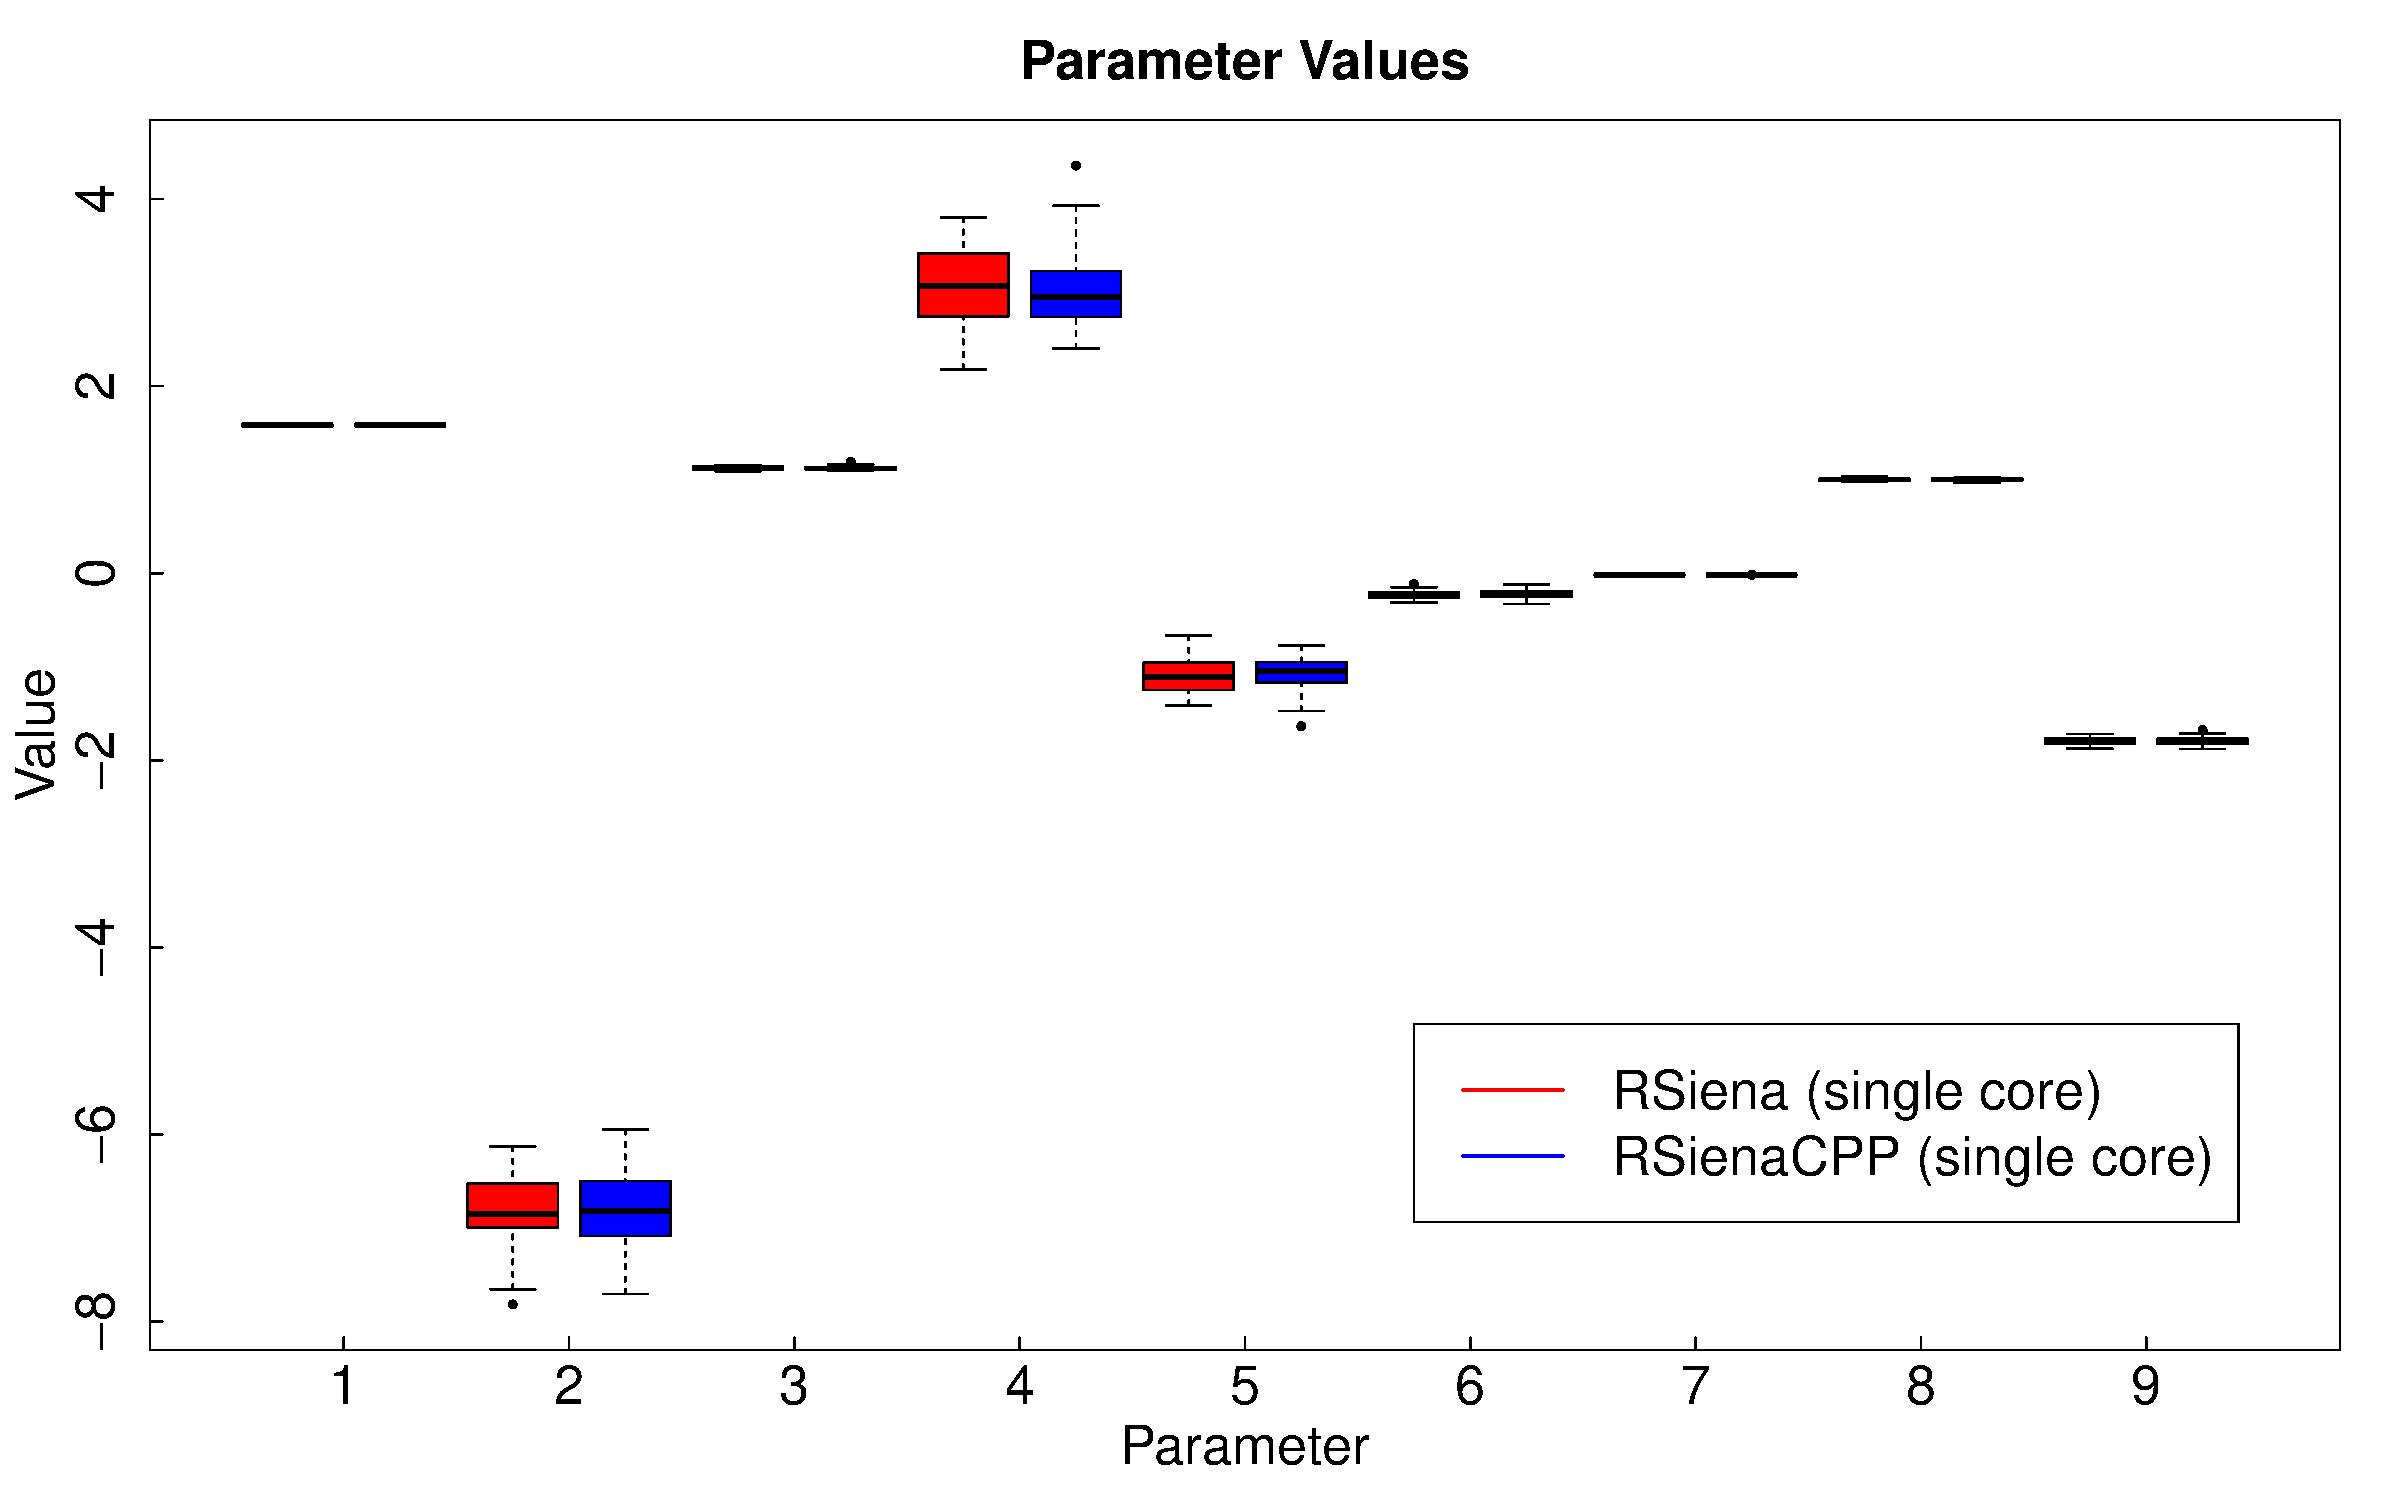
\includegraphics[width=\textwidth]{theta}
  \end{center}
  \uncover<2->{t-test: $H_0$: Difference in means equal to 0 $\to$
  Same values}
\end{frame}
\begin{frame}{Correctness}                                              % {{{1
  \begin{center}
    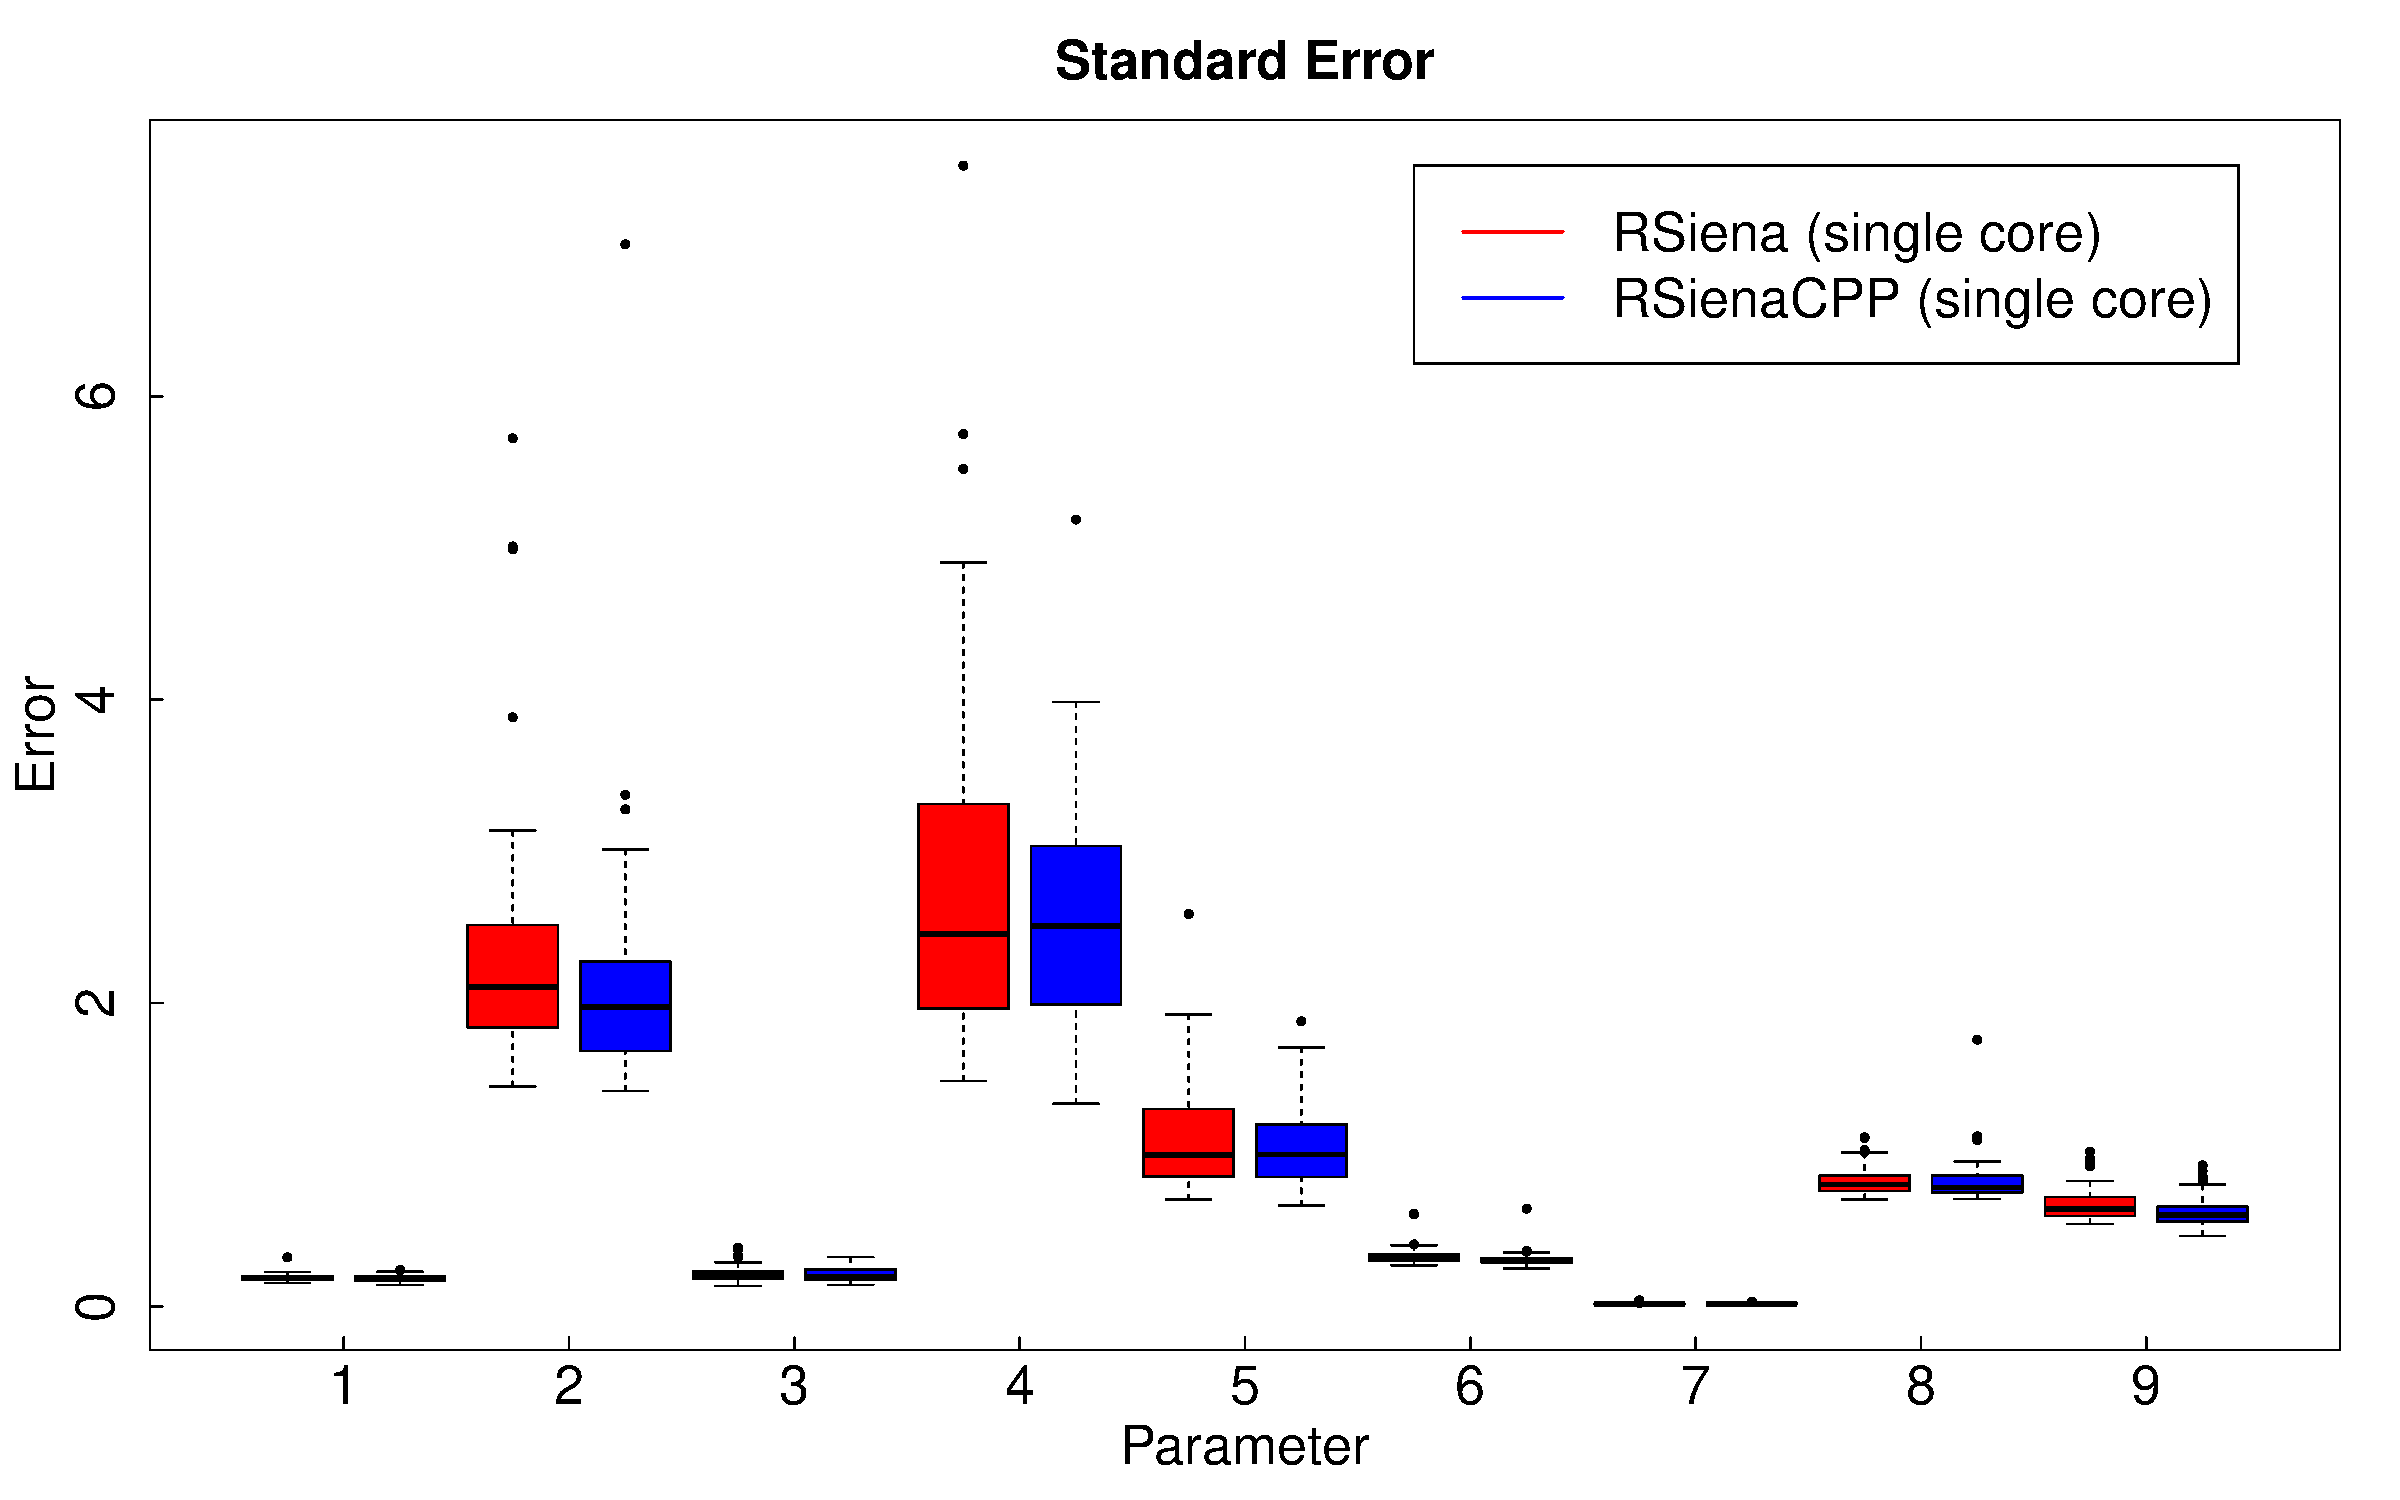
\includegraphics[width=\textwidth]{error}
  \end{center}
  \uncover<2->{t-test: $H_0$: Difference in means equal to 0 $\to$
  Same significance}
\end{frame}
\begin{frame}{Time}                                                     % {{{1
  \begin{center}
    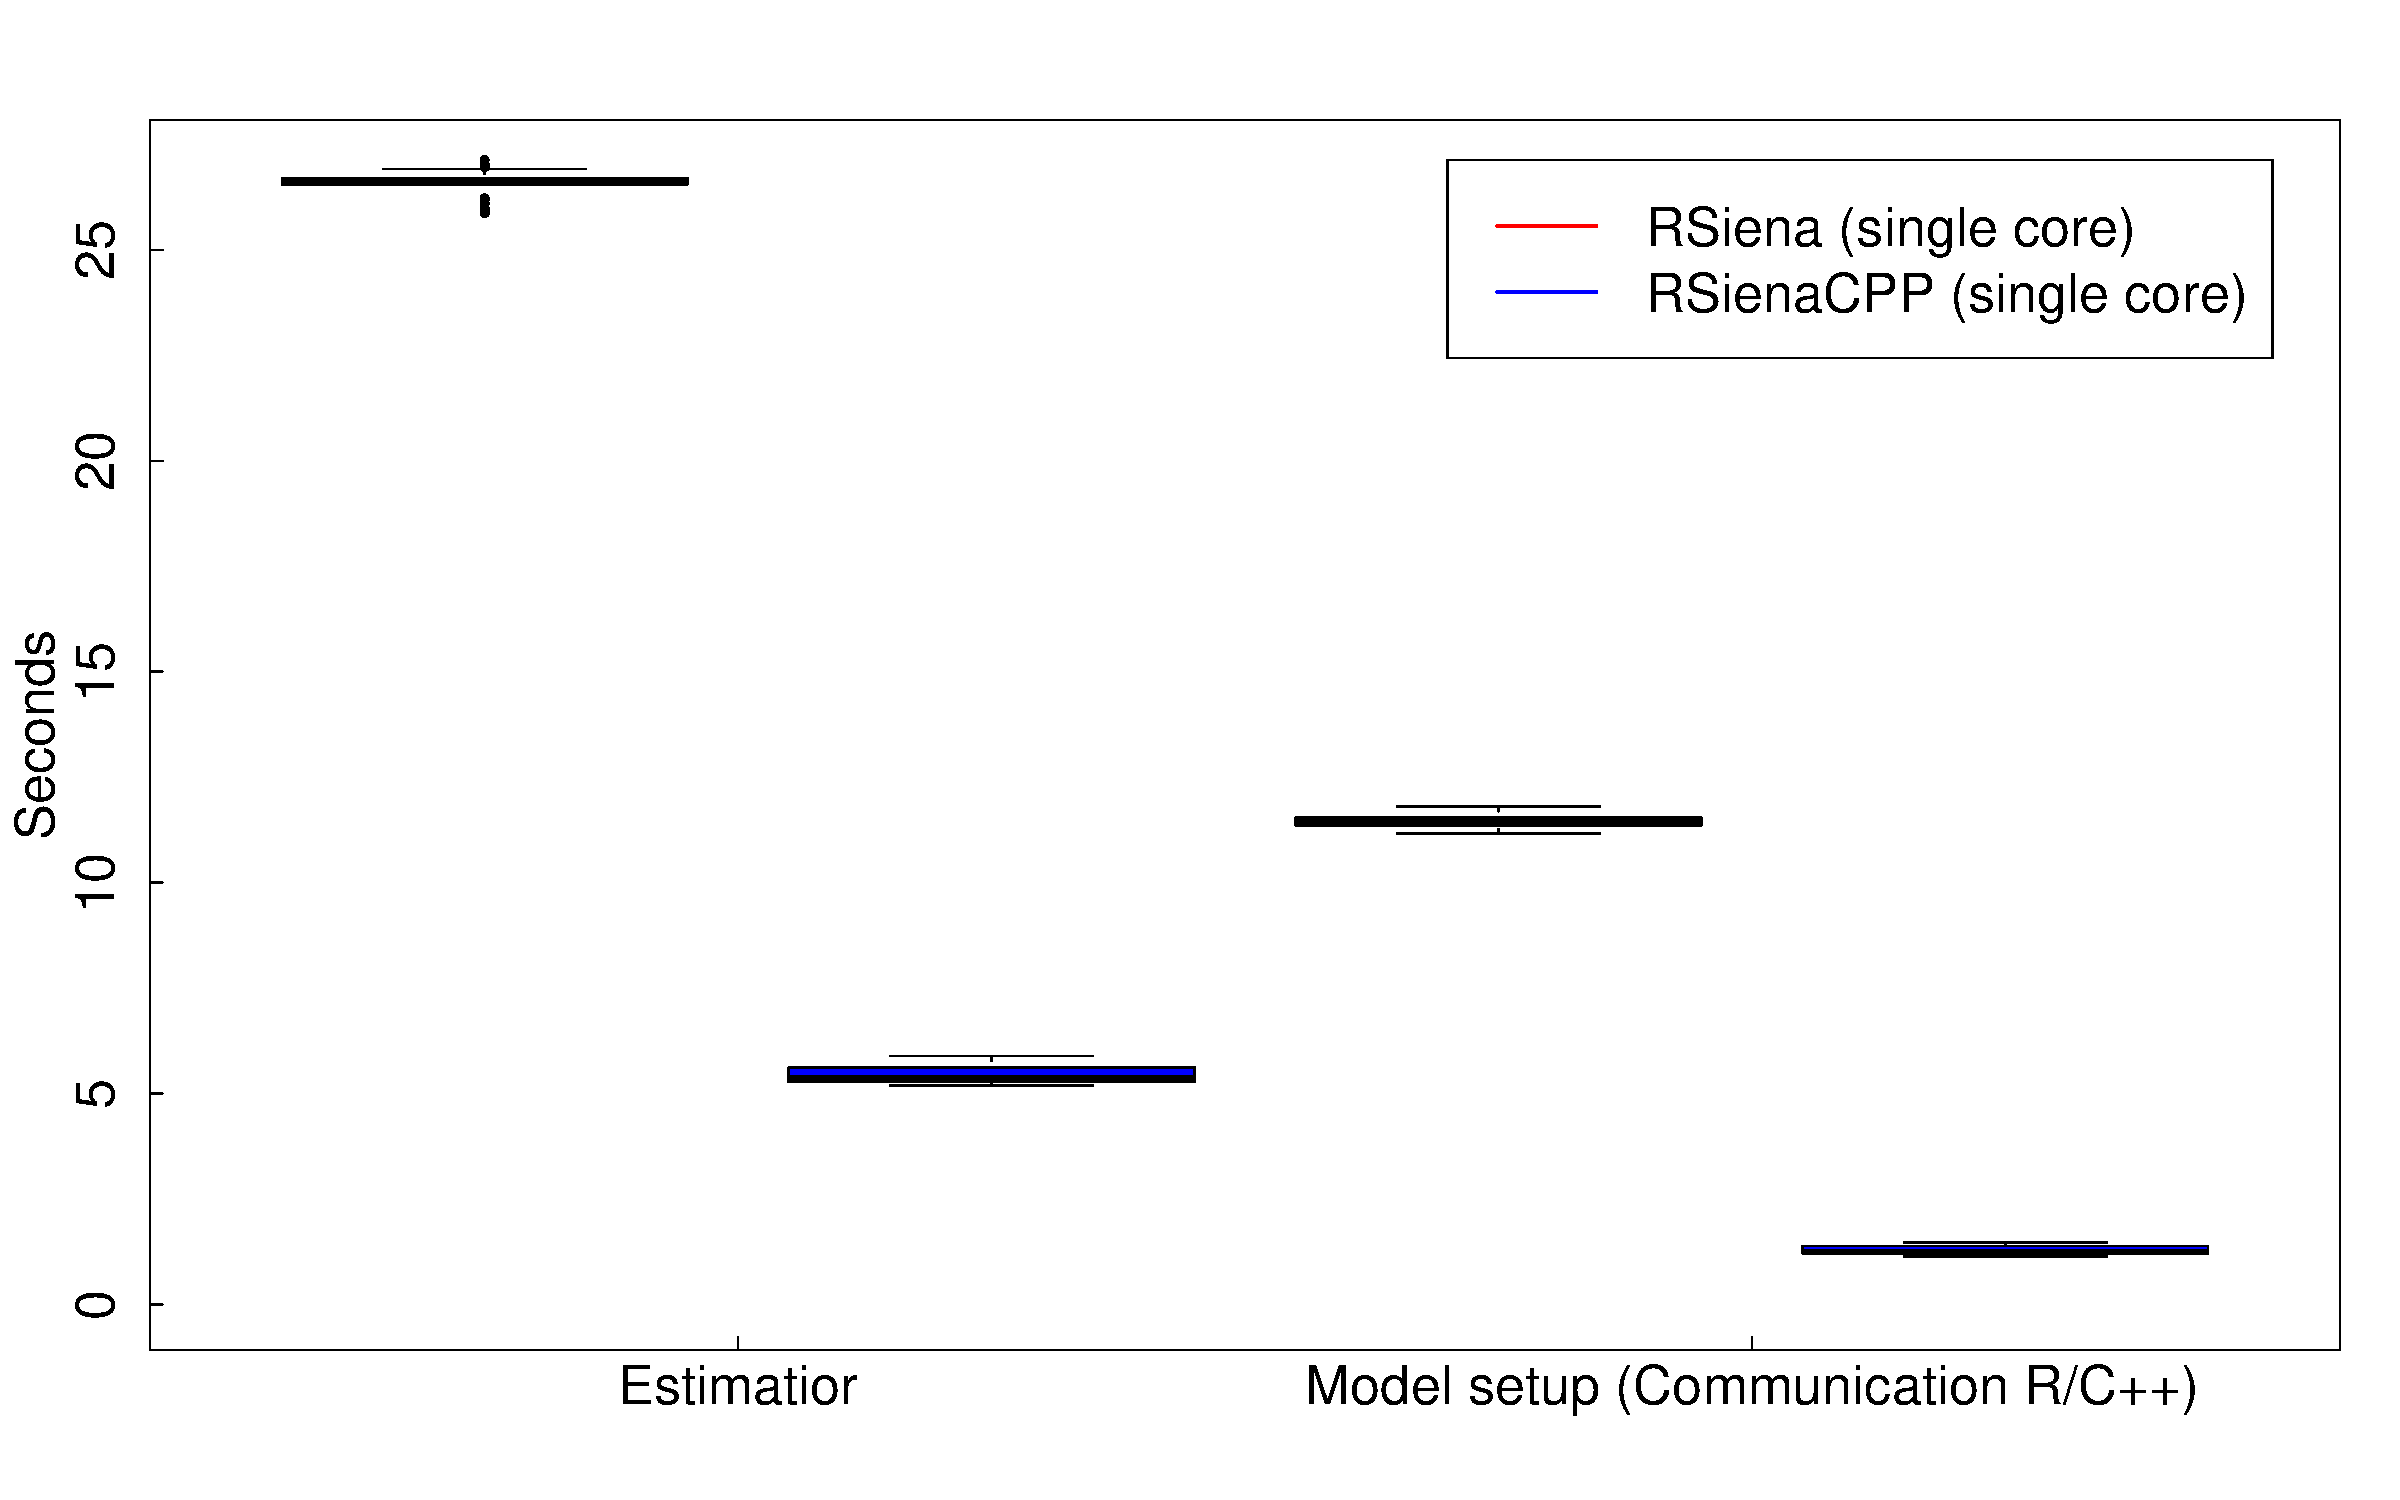
\includegraphics[width=\textwidth]{estimation}
  \end{center}
\end{frame}
\begin{frame}{Time}                                                     % {{{1
  \begin{center}
    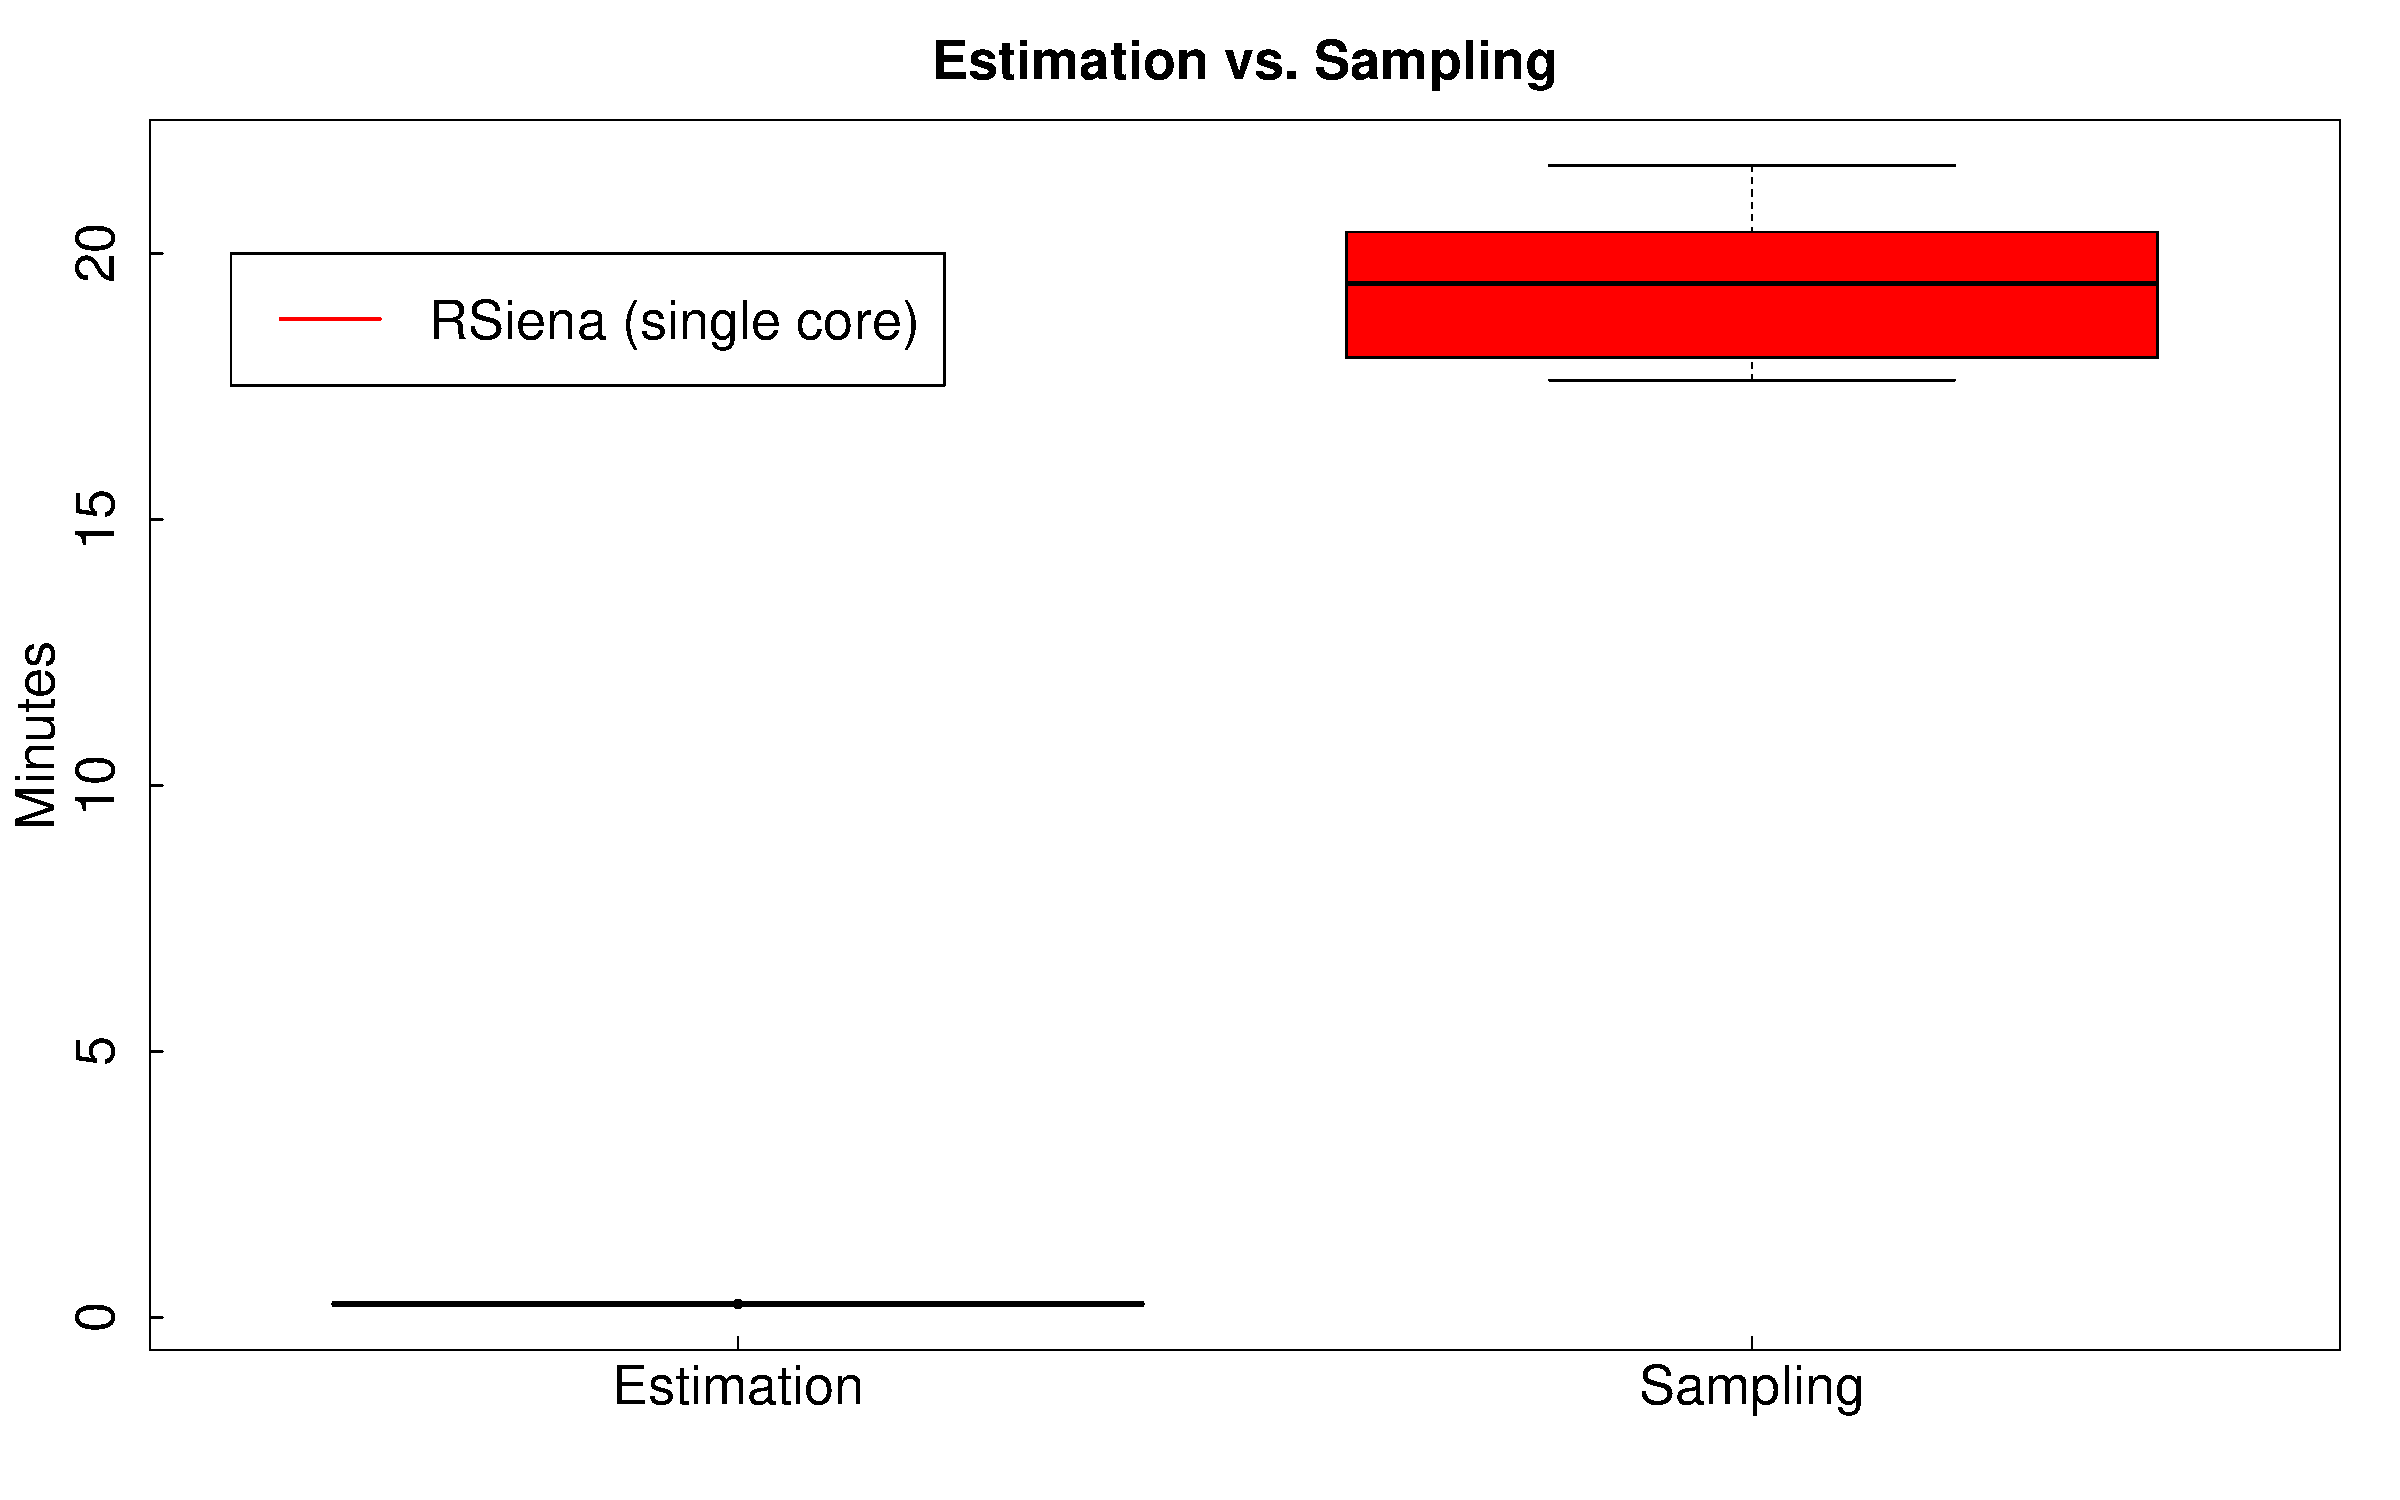
\includegraphics[width=\textwidth]{estimation-vs-simulation}
  \end{center}
\end{frame}
\begin{frame}%{iteration comparison}                                    % {{{1
  \begin{center}
    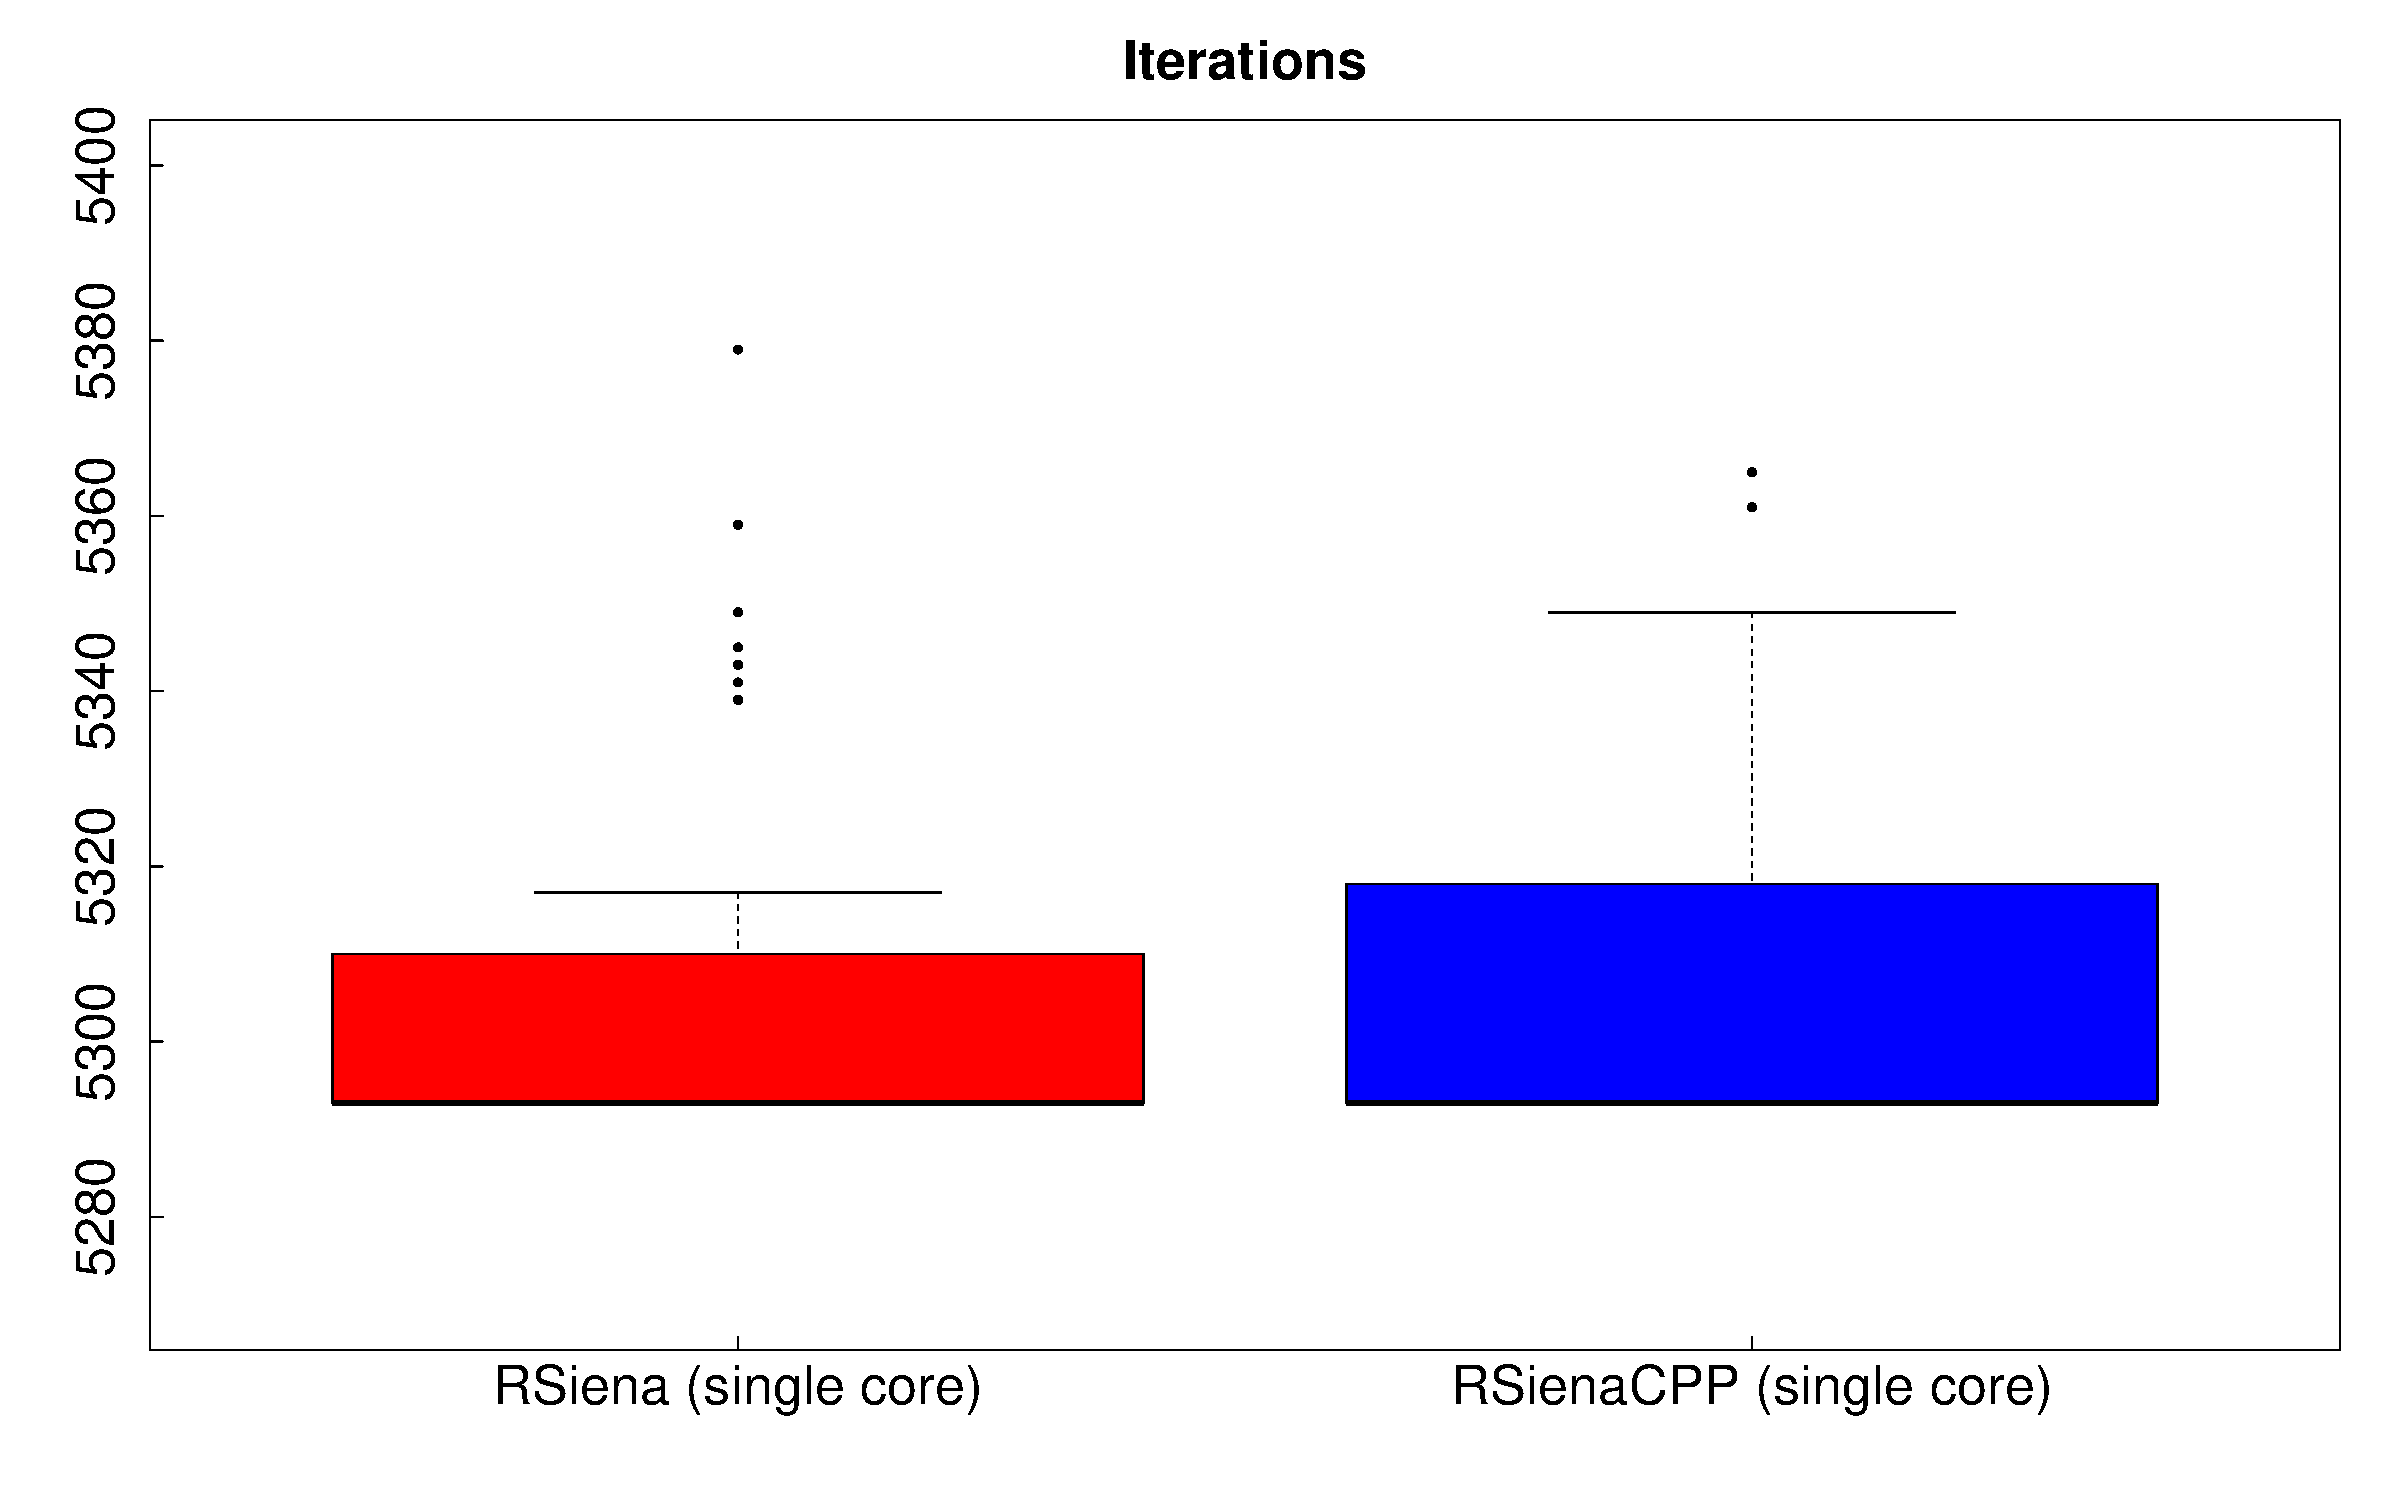
\includegraphics[width=\textwidth]{iterations}
  \end{center}
\end{frame}
\begin{frame}[fragile]                                                  % {{{1
  \begin{semiverbatim}\tiny
RSiena (single core), RSienaCPP (single core)

p-value theta
 [1] 0.86158478 0.99867274 0.22822626 0.33606423 0.37673983 0.64552216 0.04198714 0.92538597
 [9] 0.47034805 0.95480512 0.41860232 0.15292358 0.23072953 0.30079107 0.49117612 0.98786504
[17] 0.80747163 0.65988945 0.99250427 0.35462910 0.74375989 0.18145244 0.60805176 0.85317124
[25] 0.24991292 0.79829277 0.77032469 0.62140454 0.56347385 0.75473232 0.32018047 0.54956697
[33] 0.28000215 0.40919259 0.44901118 0.81716497 0.08035395 0.49786369 0.38136710 0.77346030
[41] 0.04741137 0.61756856 0.54797571 0.99022851
p-value error
 [1] 0.32025007 0.17937439 0.34329951 0.24595460 0.36017021 0.27231396 0.51909422 0.92311581
 [9] 0.04560707 0.33688985 0.46805132 0.13693804 0.82515943 0.49990828 0.55684263 0.35305619
[17] 0.79914950 0.24367384 0.32315615 0.44245695 0.43142191 0.69049199 0.19088146 0.86527129
[25] 0.56316261 0.86153612 0.55116508 0.41342449 0.69692349 0.70881414 0.53610070 0.32073280
[33] 0.43612909 0.81329017 0.37518146 0.57429171 0.49981838 0.71529054 0.06199820 0.72364385
[41] 0.58919238 0.94731312 0.99409963 0.91287258
  \end{semiverbatim}
\end{frame}
\end{document}
